\documentclass[a4paper,12pt,twoside]{report}

\usepackage{acronym}
\usepackage{url}
\usepackage{cite}
\usepackage{listings}
\usepackage[pdftex]{graphicx}
\usepackage[hang,small,bf]{caption}
\usepackage{styles/tum}
\usepackage{setspace}
\usepackage[german,english]{babel}
\usepackage{float}
\usepackage{floatflt}
\usepackage{fancyhdr}
\usepackage{color}
\usepackage{booktabs}
\usepackage[pdftex,bookmarks=true,plainpages=false,pdfpagelabels=true]{hyperref}	%TODO make yourself familiar with \label, \ref and \hyperref for referencing figures, tables, chapters, etc.
\usepackage{mdwlist}
\usepackage{enumerate}
\usepackage{array}
\usepackage{longtable}
\usepackage[utf8]{inputenc}
\usepackage[capitalize, noabbrev]{cleveref}
\usepackage{wasysym}
\usepackage{subcaption}

% Path for graphics
\graphicspath{{figures/}}

\begin{document}
\setlength{\evensidemargin}{22pt}
\setlength{\oddsidemargin}{22pt}

\def\doctype{Bachelor's Thesis}
\def\faculty{Informatik}
\def\title{Perceptual Losses for Deep Learning on Fluid Simulations}		%TODO add title in English
\def\titleGer{Perceptual Losses für Deep Learning von Flüssigkeitssimulationen}	%TODO add title in German
\def\supervisor{Prof.\ Dr.\  Nils Thürey}
\def\advisor{M.Sc.\ Georg Kohl}
\def\author{Hanfeng Wu}			%TODO add author name
\def\date{15.09.2021}		%TODO add submission / handover date


\hypersetup{pdfborder={0 0 0},
                        pdfauthor={<author>},
                        pdftitle={thesis-ba-wenjie},
                        }

\lstset{showspaces=false, numbers=left, frame=single, basicstyle=\small}

\pagenumbering{alph}

\thispagestyle{empty}

\vspace{4cm}
\begin{center}
\begin{figure}[h!]
    \centering
    
\includegraphics[width=4cm]{TUM_Logo_blau_rgb_p}
\end{figure}
\vspace{5mm}     
\huge FAKULT{\"A}T F{\"U}R INFORMATIK\\ 
\vspace{0.5cm}
\large DER TECHNISCHEN UNIVERSIT{\"A}T M{\"U}NCHEN\\
\vspace{1mm}
\end{center}

\vspace{2mm}

\begin{center}
{\Large \doctype\ in \faculty}
\vspace{10mm}

\begin{spacing}{1.5}
{\huge\bf \title}\\%[3ex]
\end{spacing}

\vspace{10mm}
{\LARGE \author}

\vspace{10mm}

\begin{figure}[h!]
\centering
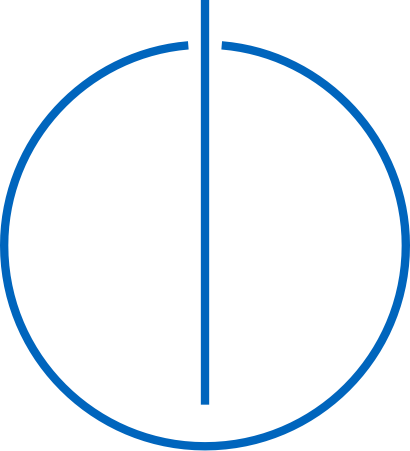
\includegraphics[width=2cm]{FAK_IN_RGB_p}
\end{figure}

\end{center}

\thispagestyle{empty}

\vspace{8mm}
\begin{center}
\oTUM{4cm}

\vspace{5mm}     
\huge FAKULT{\"A}T F{\"U}R INFORMATIK\\ 
\vspace{0.5cm}
\large DER TECHNISCHEN UNIVERSIT{\"A}T M{\"U}NCHEN\\
\end{center}

\vspace{5mm}

\begin{center}
{\Large \doctype\ in \faculty}
\vspace{8mm}

\begin{spacing}{1.3}
{\LARGE \title}\\
\vspace{8mm}

{\LARGE \titleGer}\\
\vspace{8mm}
\end{spacing}

\begin{tabular}{ll}
\Large Author:     & \Large \author     \\[2mm]
\Large Supervisor: & \Large \supervisor \\[2mm]				
\Large Advisor:	   & \Large \advisor    \\[2mm]
\Large Date:       & \Large \date
\end{tabular}

\vspace{1mm}

\begin{figure}[hb!]
\centering
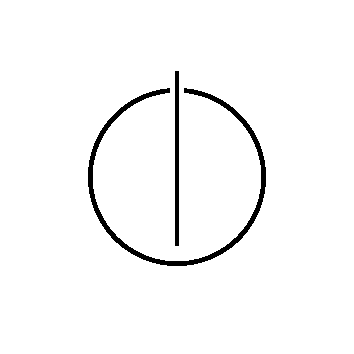
\includegraphics[width=3cm]{InformaticsLogo}
\end{figure}

\end{center}
\newpage
\thispagestyle{empty}
\mbox{}
\clearpage
\thispagestyle{empty}
\vspace*{0.8\textheight}
\noindent
I confirm that this bachelor's thesis is my own work and I have documented all sources and material used.

\vspace{15mm}
\noindent
Munich, \date \hspace{\stretch{1}} \author
\newpage

		%TODO choose one of 'diploma | bachelor's | master's thesis' in the disclaimer file

\newpage
\thispagestyle{empty}
\mbox{}

\chapter*{Acknowledgements}


\pagenumbering{roman}

\selectlanguage{english}
\begin{abstract}

%abstract english

This thesis studies the integration of perceptual loss into several models that are related to fluid simulation. Perceptual losses are used to compare high level differences, while traditional loss functions like MSE and MAE only compare the pixel level differences which is more brute force. 

Now some famous perceptual loss functions like comparing the intermediate layers of pretrained vgg network already improve its performance in some image related tasks.\cite{johnson2016perceptual} We want to show that in the context of fluid simulation, the integration of some pretrained perceptual losses should also outperform the traditional loss functions.

We tested some fluid simulation tasks in SOL\cite{um2020sol} to improve the performance of the percetual loss functions. Meanwhile we also integrate such loss functions into models like autoencoder and superresolution to compare their results with those from the same models but trained by MSE loss functions

Finally we combined the result of SOL and superresolution model to conduct some fluid simulations at a lower cost to show the advantage of integrating perceptual losses in such tasks.

\end{abstract}

\clearpage

\selectlanguage{german}
\begin{abstract}

Diese Dissertation untersucht die Integration von Wahrnehmungsverlusten in verschiedene Modelle, die sich auf die Fluidsimulation beziehen. Wahrnehmungsverluste werden verwendet, um Unterschiede auf hohem Niveau zu vergleichen, während herkömmliche Verlustfunktionen wie MSE und MAE nur die Pixelniveauunterschiede vergleichen, was roher ist.

Einige berühmte Wahrnehmungsverlustfunktionen wie der Vergleich der Zwischenschichten eines vortrainierten VGG-Netzwerks verbessern bereits seine Leistung bei einigen bildbezogenen Aufgaben.\cite{johnson2016perceptual} Wir wollen zeigen, dass die Integration einiger vortrainierter Wahrnehmungsverluste im Kontext der Fluidsimulation übertreffen auch die traditionellen Verlustfunktionen.

Wir haben einige Fluidsimulationsaufgaben in SOL\cite{um2020sol} getestet, um die Leistung der Percetual Loss Functions zu verbessern. Inzwischen integrieren wir solche Verlustfunktionen auch in Modelle wie Autoencoder und Superresolution, um deren Ergebnisse mit denen aus den gleichen Modellen zu vergleichen, die jedoch mit MSE-Verlustfunktionen trainiert wurden

Schließlich haben wir die Ergebnisse von SOL und Superauflösungsmodell kombiniert, um einige Fluidsimulationen zu geringeren Kosten durchzuführen, um den Vorteil der Integration von Wahrnehmungsverlusten in solchen Aufgaben zu zeigen.
%abstract german
\textit{Note: Insert the German translation of the English abstract here.}

\end{abstract}

\clearpage

\selectlanguage{english}


\tableofcontents
\clearpage

\clearpage

\begin{acronym}
\acro{SOL}{Solver in the Loop}
\acro{LSIM}{Learning Similarity Metrics for Numerical Simulations}

\end{acronym}

\pagenumbering{arabic}

\fancyhead{}
\pagestyle{fancy}
\fancyhead[LE]{\slshape \leftmark}
\fancyhead[RO]{\slshape \rightmark}
\headheight=15pt




%------- chapter 1 -------

\chapter{Introductions}

Our main purpose of this paper is to demonstrate the advantage of adopting the perceptual loss functions in various deep learning tasks on fluid simulation. We try to show statistically and perceptually that by integrating suitable perceptual loss functions in such tasks can outperform the original model trained on traditional loss functions such as MSE and MAE. In the end we will also compare the performance and outputs of running solely the simulation and the simulation combined with some deep learning models.
\section{Fluid simulation}
\subsection{Navier Stokes Equation}
The state of art Fluid simulation is based on the famous incompressible equation Navier-Stokes equation

\begin{equation}
\frac{\partial \vec u}{\partial t}+\vec u\cdot \nabla\vec u+\frac1\rho\nabla p = \vec g + \nu\nabla\cdot\nabla\vec{u}
\end{equation}

\begin{equation}
{\nabla}\cdot\vec{u} = 0
\end{equation}

where $\nabla$ denotes the gradient, $\nabla\cdot$ denotes the Divergence, $\vec{u}$ denotes the velocity of the fluid, $t$ denotes the time step, $\rho$ denotes the density of the fluid, $p$ denotes the pressure, $\vec{g}$ denotes the gravity and $\nu$ denotes the viscosity of the fluid.

The equation (1.1) is actually a transformation of the $\vec{F} = m\vec{a}$ and the equation (1.2) describes the incompressibility of the fluid.
\subsection{Grid Stucture}
The way of storing the velocity and the density is based on two different grid structure. We store the dencity in the center of each cell, we call it centeredgrid or scalar grid. However for storing the velocity, we sample them at the face centers of each cell\cite{doi:10.1063/1.1761178}. In such way we can more easily compute the inflow and outflow of each grid for each direction, however as a trade off, the data format would be more complex than normal centeredgrid, and we usually have to stack each verlocity array of each dimension together and also adopt them individually in some computations(e.g. computing loss function in deep learning)

\begin{figure}[h]
\centering
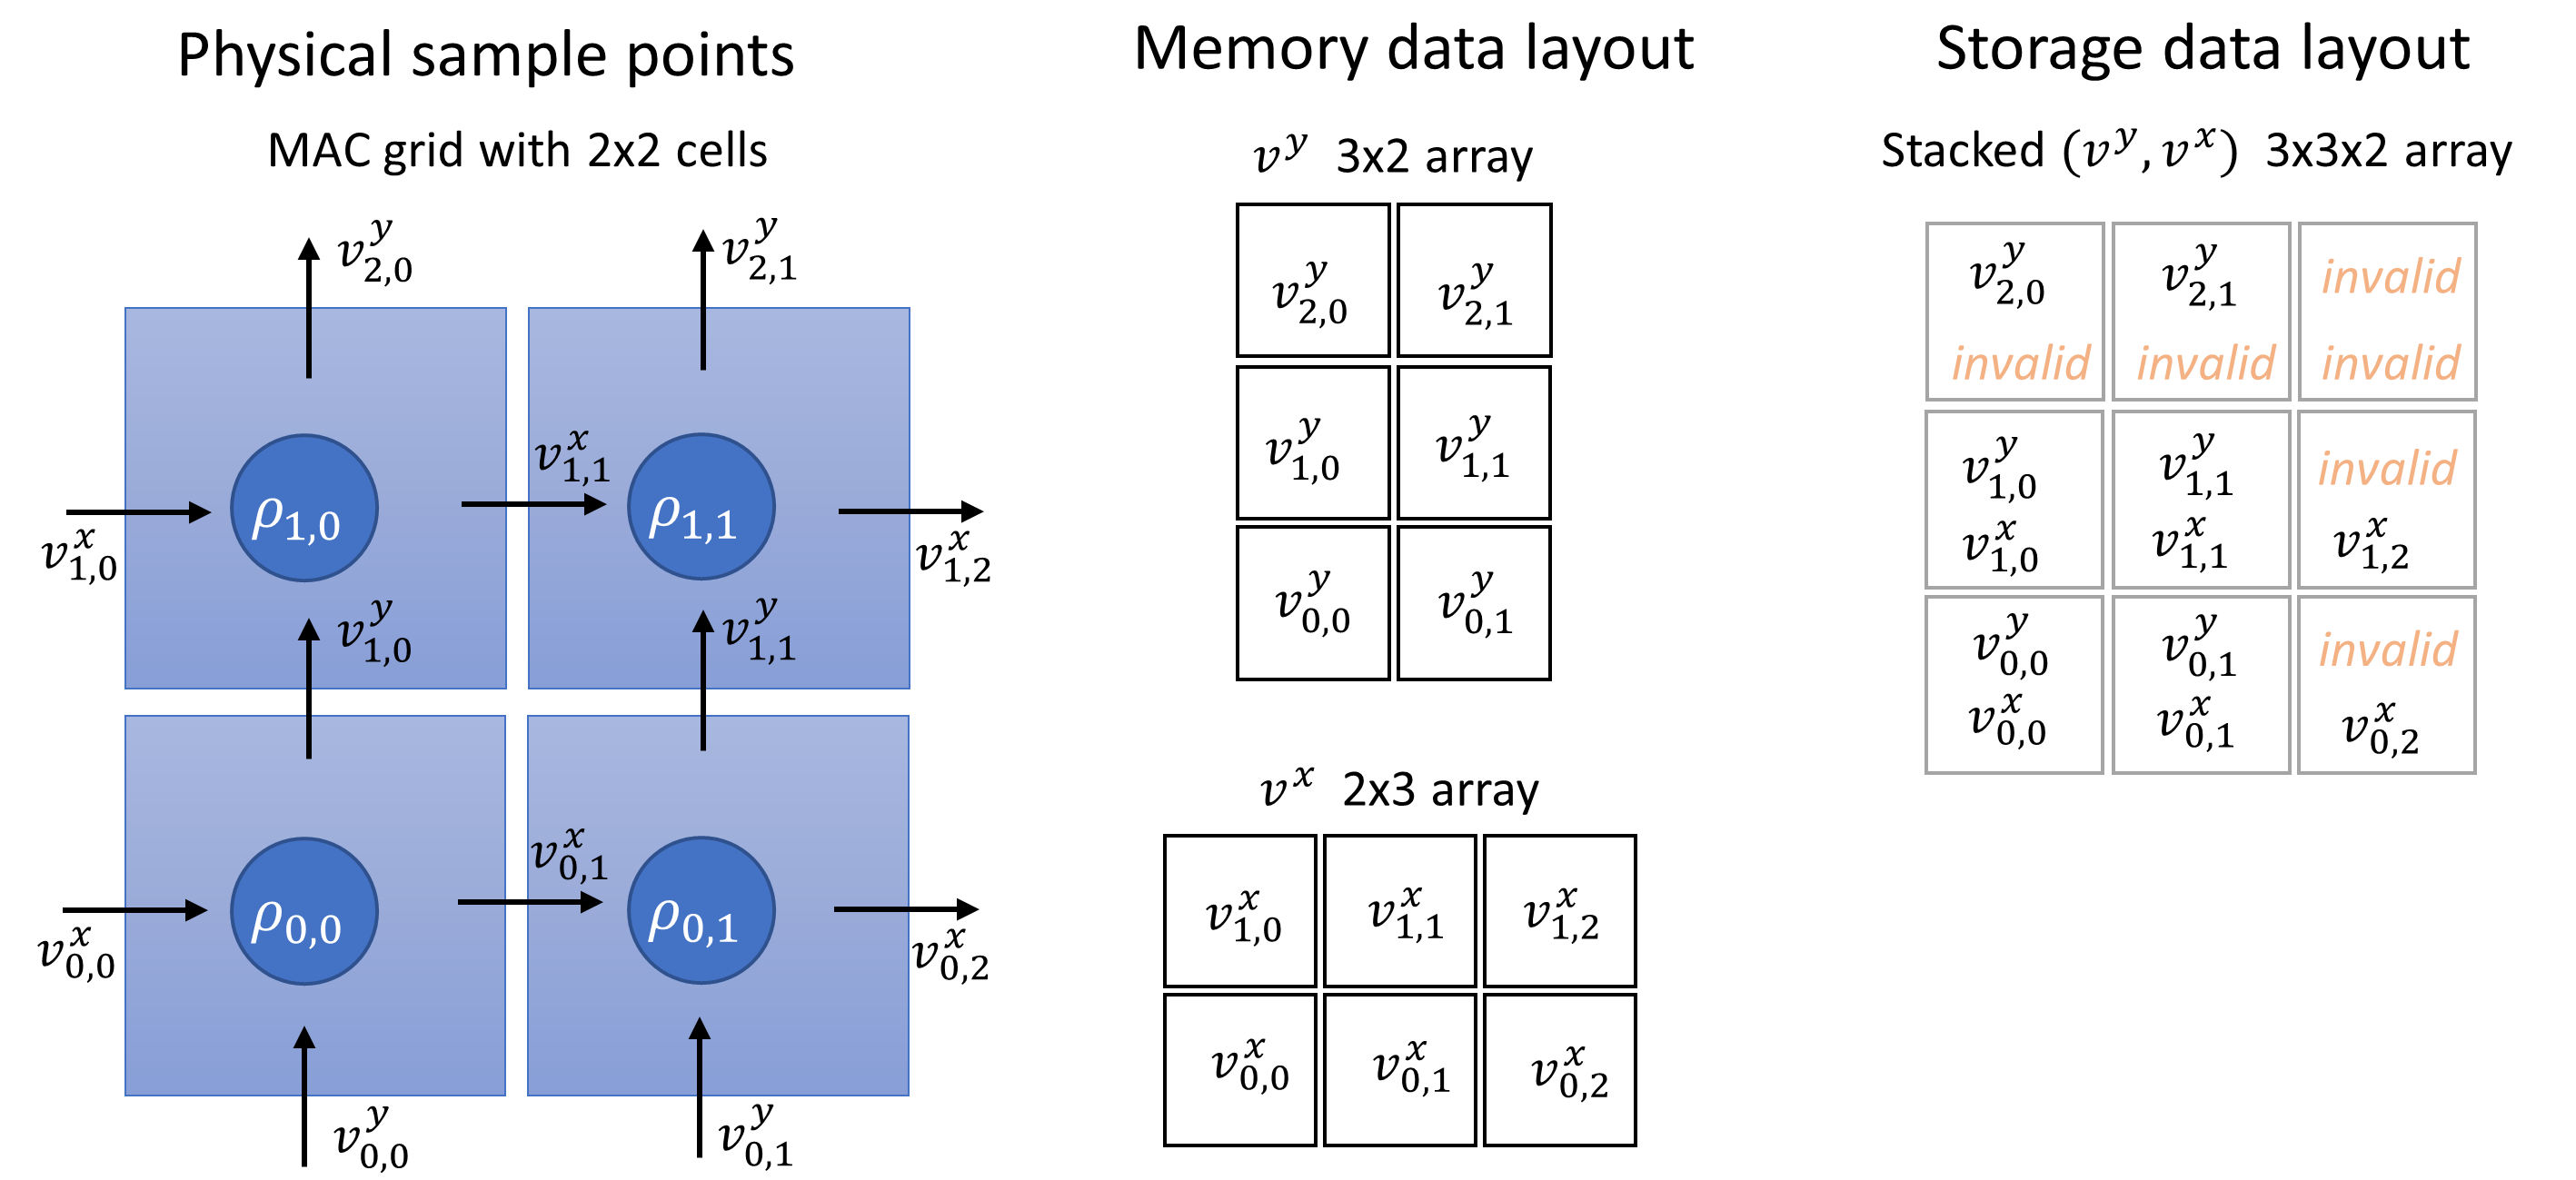
\includegraphics[width=\textwidth]{Staggered.png}
\caption{Staggered grid format}
\end{figure}

\subsection{Advection}
With the knowledge base of the NS-equation and grid structures we now need the advection algorithm to run the simulation. We adopt the semi-lagrangian advection algorithm. In the lagrangian point of view, if we want to compute the grid value of the n+1 time step of grid position $\vec{x_G}$, we should figure out which particle actually flows to the grid $\vec{x_G}$ from time step n+1. If we name the grid position of the particle as $\vec{x_P}$, then the new particle at time step n+1 in $\vec{x_G}$ should have the same physical property as the particle at time step n in $\vec{x_P}$

\begin{figure}[h]
\centering
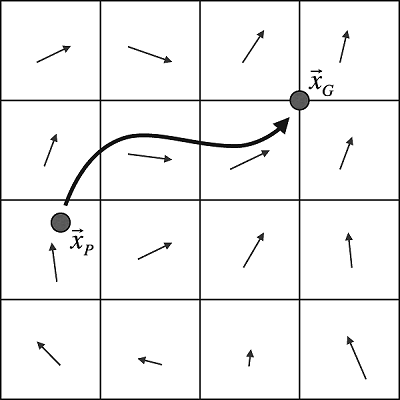
\includegraphics[scale=0.5]{advection.png}
\caption{advection}
\end{figure}

we first use the euler equation to calculate the $\vec{x_P}$ as a step before of $\vec{x_G}$
\begin{equation}
\vec x_P=\vec x_G-\Delta t\frac{d\vec x_G}{dt}
\end{equation}

because $\frac{d\vec x}{dt}=\vec u(\vec x)$ we have

\begin{equation}
\vec x_P=\vec x_G-\Delta t\vec u(\vec x_G)
\end{equation}
where $\vec u(\vec x_G)$ denotes the velocity sampled at the position $x_G$, with the advection we can update the velocity, pressure and density of the whole vector field.

with all the knowledge above, we can formulate a sequence to conduct the basic fluid simulation.

$\\\bullet$ start with an initial velocity field $\vec{u}^{0}$ with the property ${\nabla}\cdot\vec{u} = 0$
$\\\bullet$ choose a time step $\Delta t$ 
$\\\bullet$ For time step n = 0, 1, 2, ...
\par$\bullet$  $\vec{u}^{A} = advect(\vec{u}^{n}, \vec{u}^{n}, \Delta t)$
 \par$\bullet$  add the extra force $\vec{u}^{B} = \vec{u}^{A} + \Delta t\vec{g}$
 \par$\bullet$  $\vec{u}^{n+1} =make\_incompressible(\Delta t, \vec{u}^{B})$


\section{Deep learning tasks}
There are also various ways of integrating deep learning models into the fluid simulation.
\subsection{Autoencoder}
The Autoencoder model has a bottle neck shape, which aims to produce the same output as the input. Once trained, the Autoencoder model can be saparated into two parts, namely the encoder and the decoder, which can compress the image with the encoder and later decompress the image with the decoder to its forer shape.
\subsection{Superresolution}
With the superresolution model, we can upscale the low-resolution images to high-resolution images, which based on that we have fed lots of similar data to the model. In this paper, we apply the Superresolution model at the end of the Solver in the Loop model in order to boost the fluid simulation while still obtain a fairly similar output.
\subsection{Solver in the Loop}
When we want to perform our fluid simulation on a lower-resolution domain to decrease the time cost, we always suffer from the numerical error comparing to the simulation running on the higher-resolution domain. It is reasonable because with the same initial state, the vector field on the higher domain has richer information than the one sampled in the lower domain. Dr.\ Kiwon Um\cite{um2020sol} developed a mechanisim to learn the difference between the 2 different domains to reduce the numerical error.

\section{Perceptual loss functions}
Perceptual loss functions are used when comparing two images, they are not like traditional loss functions like MSE or MAE which only computes the low level pixel differences. Perceptual losses on the other hand, are normally forward networks trained for specific tasks. For example, VGG-16 network was trained for massive image classification, and LSIM was trained on smoke and fluid simulations. When adopting those networks, we can either compute the mse loss between the intermediate layers of the trained network, or directly passing it through depending on the goal of the chosen perceptual loss network. These perceptual loss networks tries to retrieve the high level differences between the images, hence will usually have a better performance than the traditional loss functions. In a word, traditional loss functions have more general use cases, while perceptual loss functions will achieve better performance on specific tasks.
In this paper we mainly focus on comparing the performance between traditional loss function MSE and perceptual loss functions LSIM, VGG-16 and lpips.




\chapter{Related Work}
similar goal area methods


%------- chapter 2 -------

\chapter{Metrics and Perceptual Losses}

In this chapter we will cover several loss functions that we adopted in this paper and briefly explain their characteristics and their drawbacks. More percise integrations and results will be convered in the chapter 5.

\section{Mean Squre Error}

MSE is one of the most widely used loss functions.
\begin{equation}
{MSE}=\frac{1}{n}\sum_{i=1}^n(Y_i-\hat{Y_i})^2
\end{equation}
Where ${Y}$ is the reference tensor and $\hat{Y}$ is the predicted tensor based on the trainable parameters. With this loss function being adopted, the network will try to do the gradient decent on the weights in a way that can achieve minimum square error. The optimal case is that the predicted tensor $\hat{Y}$ is exactly the same is the reference tensor ${Y}$. We can see that the core idea for the MSE is very general so that this loss function can be applied almost for any models, however the MSE loss function is not suitable for some image related tasks. If the two inputs of the MSE loss function is merely a image with its core content shifted by some pixels, the MSE will produce a very high value, which is not representitive, in another word, the MSE does not have shift or rotate invariance. 

Besides, MSE computes the squre error of the two tensors, which means that MSE is also prone to the outliers, beacause when it has a very large outlier in the tensor, the result of MSE loss function will be strongly influenced, so in most image construction cases, in order to achieve a lower square error, the output will be a relative blur one compared with the original.
\begin{figure}
\centering
\begin{subfigure}{0.4\textwidth}
  \centering
  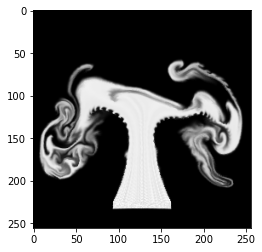
\includegraphics[scale=0.5]{MSEref.png}
  \caption{ref}
\end{subfigure}
\begin{subfigure}{0.4\textwidth}
  \centering
  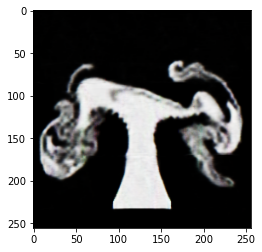
\includegraphics[scale=0.5]{MSEblur.png}
  \caption{MSE output}
\end{subfigure}
\end{figure}

\section{Learning Similarity Metrics for Numerical Simulations}

LSiM \cite{kohl2020learning} is a neural network-based approach that computes a stable and generalizing metric. Due to the unreliability of the MSE loss in numerical simulation tasks, LSiM has been established. It aims to demonstrate the performance of CNN-based evaluations on numerical simulation tasks. The data used to train LSiM are generated with known partial differential equations (PDEs)

\begin{figure}
\centering
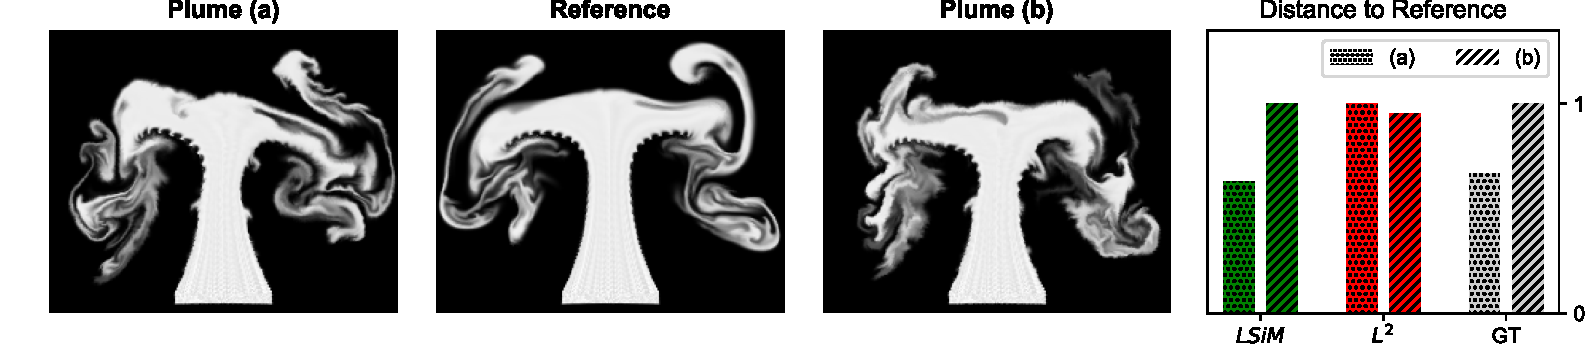
\includegraphics[scale=0.5]{Plumes.pdf}
\caption{Comparison}
\end{figure}

\section{VGG-16 loss network}

\textit{Note: This section would summarize the architectural style Representational State Transfer (REST) using definitions, historical overviews and pointing out the most important aspects of the architecture.}

\section{Lpips}




%------- chapter 3 -------

\chapter{Datasets}

\section{Autoencoder}


\section{Superresolution}

\section{Solver in the Loop}





%------- chapter 4 -------

\chapter{Tasks and Experiments Setup}

\section{Autoencoder}

\section{Superresolution}

\section{Solver in the Loop}



%------- chapter 5 -------

\chapter{Results and Analysis}

\section{Comparison}

\subsection{Numerical evaluation}

\subsection{Time cost evaluation}

\section{Limitaions}





%------- chapter 6 -------

\chapter{Conclusion}
\section{Future work}
\section{Summary}






\appendix

\chapter{e.g. Questionnaire}

\textit{Note: If you have large models, additional evaluation data like questionnaires or non summarized results, put them into the appendix.}


\clearpage

\listoffigures
\clearpage

\listoftables
\clearpage

\bibliography{thesis}
\bibliographystyle{alpha}

\end{document}
